%\section{Примеры численного моделирования стабилизации}
\section{Примеры численного моделирования стабилизации}


\vspace{1em}

\newtheorem{exmp_st}{Пример}

\begin{exmp_st}
\end{exmp_st}

В качестве начальных условий возмем $u_0 = \sin(\pi x)$. Продемонстрируем 
стабилизацию системы при $\alpha = \pi^2 + 0.1$. Фиксируем $\omega = (0, 0.2)$. 
Необходимо подобрать параметры $m$, $r_m$ так, чтобы $\beta > 0$ и $q > 0$. 
Рассмотрим подробнее $q = [(\pi(m + 1))^2 - \alpha - 1]$. При заданном 
$\alpha = \pi^2 + 0.1$, достаточно взять $m = 2$ для выполнения неравенства. 
Параметр $r$ придется подобрать так, чтобы решение стремилось к нулю.


\begin{figure}[H]
    \centering
    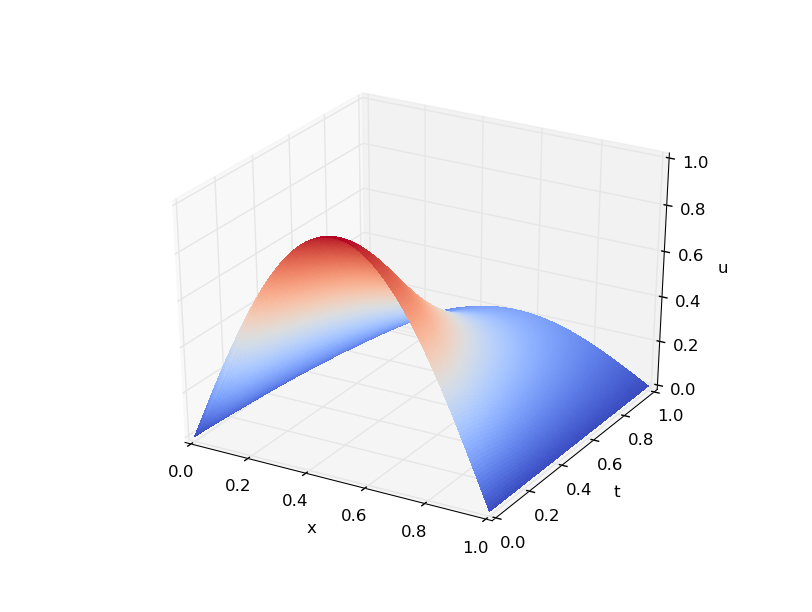
\includegraphics[width=4in]{par_re_pi01}
    \caption{Управление $\omega = (0, 0.4),\; m = 2,\; r = 8$}
    \label{fig:fig03}
\end{figure}

\begin{exmp_st}
\end{exmp_st}

Пусть $u(x, 0) = x(1 - x)$ - начальное условие . Заведомо выберем параметр 
$\alpha = \pi^2 + 3$ большим. Зафиксируем $\omega = (0, 0.4)$. 
Необходимо подобрать $m$, таким чтобы $q > 0$. При $m \ge 2$ условие выполняется, 
поэтому мы фиксируем $m = 2$. На рис.~\ref{fig:fig04} показано, как быстро растет решение 
задачи \eqref{sys} - \eqref{s_control} при небольшом увеличении $\alpha$. 
Стабилизация этой системы представлена на рисунке 5

\begin{figure}[H]
    \centering
    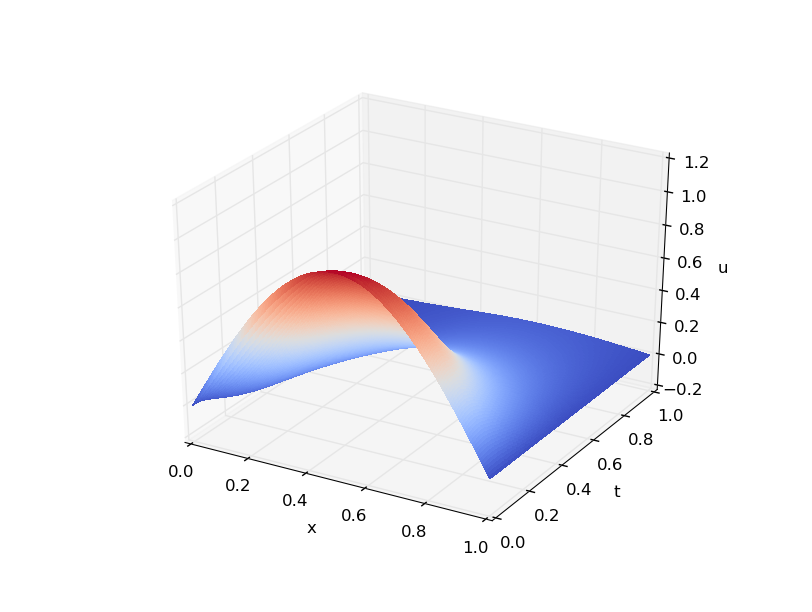
\includegraphics[width=4in]{par_re_pi3}
    \caption{Управление $\omega = (0, 0.4),\; m = 2,\; r = 15$}
    \label{fig:fig04}
\end{figure}
